\documentclass{article}

%\usepackage[latin9]{inputenc}
\usepackage{amsmath}
\usepackage{graphicx}
\usepackage{algorithmic}
\usepackage{stfloats}
\usepackage{hyperref}

%Common packages.
\usepackage{cite}
\usepackage{amsmath}
\usepackage{amssymb}
\usepackage{graphicx}
\usepackage{listings}
\usepackage{url}
\usepackage{appendix}
\usepackage{adjustbox}

%NOT TO BE INCLUDED IN SUBMISSION.
\usepackage{hyperref}

%Need to be at last.
\usepackage{cleveref}


\PassOptionsToPackage{hyphens}{url}\usepackage{hyperref}

\title{On the Insecurity of the Randomness Generation in a Large Class of Commercial IoT Devices.}

\author{ 
Yan Yan \\ 
%Department of Computer Science, \\ 
%University of Bristol, UK \\ 
y.yan@bristol.ac.uk
\and
Elisabeth Oswald \\ 
%Department of Computer Science, \\ 
%University of Bristol, UK \\ 
Elisabeth.Oswald@bristol.ac.uk
\and
Theo Tryfonas \\ 
%Department of Civil Engineering, \\ 
%University of Bristol, UK \\
Theo.Tryfonas@bristol.ac.uk
}

\date{University of Bristol, \\ UK \\ \today}

\begin{document}

\maketitle

%\tableofcontents
\begin{abstract}
Smart metering, smart parking, health, environment monitoring, and other applications drive the deployment of the so-called Internet of Things (IoT). Whilst cost and energy efficiency are the main factors that contribute to the popularity of commercial devices in the IoT domain, security features are increasingly desired. Security features typically guarantee authenticity of devices and/or data, as well as confidentiality of data in transit. Our study finds that whilst cryptographic algorithms for confidentiality and authenticity are supported in hardware on a popular class of devices, there is no adequate support for random number generation available. We show how to passively manipulate the on-board source for randomness, and thereby we can completely undermine the security provided by (otherwise) strong cryptographic algorithms, with devastating results. 
\end{abstract}

\section{Introduction}
Applications for IoT flourish, leaving a great desire for not only energy efficient, cheap devices, but also for devices that support basic cryptographic functionality such as confidentiality and/or authenticity. Popular algorithms are e.g. the Advanced Encryption Standard\cite{AES} (AES) for confidentiality, and the Elliptic Curve Digital Signature Algorithm\cite{ECDSA} (ECDSA) for authenticity, which, when used in conjunction, enable applications to establish secure end-to-end channels via e.g. Datagram TLS\cite{DTLS} (DTLS). 

However whilst AES is a secure block cipher, one might require randomness to turn it into a secure encryption scheme for arbitrary length messages. Somewhat similarly, ECDSA relies on a known-to-be-secure mathematical problem. However, it also requires large and securely generated random numbers. Consequently, when supporting cryptography the secure generation of random numbers is crucial. 

%The prospering IoT applications constantly proposes higher requirements to security where cryptography plays an important role. Among all prerequisite of implementing cryptographic primitives on these IoT devices, a reliable Random Number Generator (RNG) is critical as it is required in most cryptographic algorithms. In practice, a RNG typically involves a Pseudo Random Number Generator (PRNG) seeded by a high entropy physical source.

In 2013, Texas Instruments (TI) launched a new System-on-chip (SoC), the CC2538\cite{CC2538}, featuring secure channels over 802.15.4 via multiple cryptographic hardware accelerators. Partially because of these cryptographic accelerators, projects such as Contiki\cite{Contiki} and OpenWSN\cite{OpenWSN} began to support the CC2538 with enthusiasm. As of writing this paper, the chip features in the suggested list for Zigbee and 6LoWPAN solutions on TI's website\cite{ZigbeeProducts}.

However, despite all the cryptographic hardware support, the CC2538 does not have a Random Number Generator (RNG) dedicated for cryptographic applications; instead, the user's guide suggests to use a 16 bit Linear Feedback Shift Register (LFSR) as a Pseudo RNG (PRNG) where the seed is generated by the Radio Frequency (RF) module sampling from the radio noise. Whilst the user guide at no point suggested that this method should be used in conjunction with cryptographic algorithms, developers have little choice in the absence of alternatives. Also, in the absence of published attacks, there is often a temptation to ignore warnings towards insecure RNG implementations such as in \cite{SmartMeterBlog}. 

\subsection{Our Contribution}
We show in this study that this choice proves catastrophic for cryptographic applications, not only because the in-built PRNG has only 16 bit entropy which can be easily predicted, but also because we are able to practically demonstrate how to bias the seed obtained from the RF module through the RF interface. Consequently, even if the weak in-built PRNG was replaced by a stronger component, the source for the seed could still be tampered with and thus render the system insecure. All the experimental work in this paper are performed on the latest Contiki release version 3.0.
%The related source code can be accessed at \cite{prngtest}.

Our paper is structured as follows. We begin in \Cref{ContikiDriverIssue} with some Contiki RNG driver issues for CC2538. \Cref{LFSR} revises why using a 16 bit LFSR as PRNG is a bad practice and we show how this design flaw can be exploited to break DTLS in \Cref{BreakDTLS}, before reviewing the problem in \Cref{PRNGReflection}. In \Cref{Seed} we explain how CC2538 samples the radio noise into random seed and then we demonstrate a bias attack in \Cref{Jamming} which could be achieved given physical access to the device. Finally we conclude the paper in \Cref{Conclusion}.

\subsection{Related Work}
The design flaw of using a 16 bit LFSR as PRNG has been reported by \cite{SmartMeterBlog}\cite{CC2530PRNG} on CC2430\cite{CC2430Manual} and CC2530\cite{CC2530Manual} respectively. These chips are the predecessors of CC2538 in the SimpleLink\texttrademark  series and they all adopted the same RNG design. The blogs reported the flaw and warned that it could easily be exploited to compromise the Z-Stack library\cite{ZStack} and Smart Energy Profile ECC in many Smart Meter applications. We essentially `rediscovered' that this poor design choice still features in the CC2538 product. However, whilst in previous work the possibility of injecting a jamming signal was contemplated, we are the first to actually examine the technical feasibility of this and to demonstrate a working attack.

\subsection{Contiki Driver Issues}\label{ContikiDriverIssue}
We made extensive use of Contiki in our research and fixed (and reported) some coding issues in the CC2538 RNG driver (Contiki release-3.0). These were, the reading out of the LFSR without ready check, a lack of validity check when reading random seed bits from the RF module, and a bug that drops the Most Significant Bit (MSB) and leaves the Least Significant Bit (LSB) to be constantly zero in the seed.  We modified the code and fixed these issues in our experiments. 

Another issue in the driver is that the CC2538 User's Guide\cite{CC2538Manual} suggests only to use the lower byte (8 bits) as a random number but the driver actually used 16 bits in the LFSR. However, this coding mistake does not affect our result, as will be explained in  later sections.
\section{High Level PRNG Design and its Implication on DTLS Security} \label{LFSR}
We begin this section by reviewing how the 'default' PRNG (as provided by the CC2538) turns a seed into a stream of pseudo random numbers using a 16-bit LFSR (see CC2538 User's Guide\cite{CC2538Manual} Section 16.1). The polynomial that defines the feedback function is given as $x^{16} + x^{15} + x^{2} + 1$ which corresponds to the well known CRC16 schem\cite{CRC}. When used as a PRNG (after it has been seeded), the input bit is simply set to zero. The CC2538 User's Guide\cite{CC2538Manual} gives clear instructions on how to use the LFSR: by setting specific control bits to 01, the LFSR performs 13 CRC16 operations and its content can be read out as a random number. 


% describes the PRNG design \begin{quote}
%The random-number generator is a 16-bit linear-feedback shift register (LFSR) with polynomial X 16 + X 15 +
%X 2 + 1 (that is, CRC16). It uses different levels of unrolling depending on the operation it performs. The basic version (no unrolling) is %shown in Figure 16-1 (\Cref{CRC16} in this paper). \end{quote}

%\begin{figure}[!t]
%\centering
%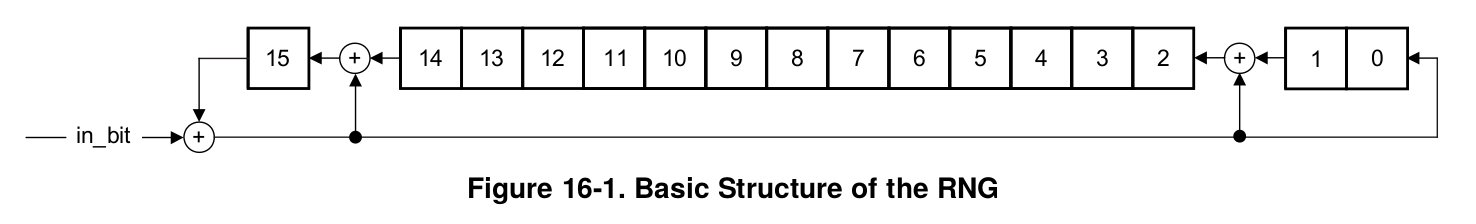
\includegraphics[width=2.5in]{fig/crc16.png}
%\caption{CRC16 LFSR, from CC2538 User's Guide}
%\label{CRC16}
%\end{figure}

%When used as a PRNG, the in\_bit in \Cref{CRC16} is constantly $0$. The Contiki driver calls the PRNG by: (Section 16.2.1in CC2538 User's Guide)
%\begin{quote}
%Another way to update the LFSR is to set the RCTRL bits in the SOC\_ADC\_ADCCON1 register to 01. This clocks the LFSR once (13x unrolling), and the RCTRL bits in the SOC\_ADC\_ADCCON1 register automatically clear when the operation completes.
%\end{quote}

%In another word, the LFSR is updated by performing 13 CRC16 operations in \Cref{CRC16} upon each RNG call. Since the CRC16 is deterministic and the register has only $16$ bits, the PRNG can be modelled as a Deterministic Finite Automaton (DFA) which made its output easily predictable as we will explain later in this section.

Formally, because there are only 16 bits in the LFSR, we can denote the universal set of its  possible values (or called states) $\mathbb{S}$ as:
\begin{equation} \label{PRNGState}
\mathbb{S} = \{ S_{i} | S_{i} \in \{2\}^{16}\}
\end{equation}
\Cref{PRNGState} implies that the LFSR can have no more than $|\mathbb{S}| = 2^{16} = 65536$ states.

We denote the LFSR update operation as:
\begin{equation}
F:\mathbb{S} \rightarrow \mathbb{S}
\end{equation}
where $F$ is $13$ times of CRC16 operation on the current state according to the manual.

Denote the 16 bits random seed sampled by the radio noise as $S^*$. The PRNG output can be formalised as:
\begin{equation}
	\begin{aligned}
	S_{0} &= S^* \\
	S_{i+1} &= F(S_{i})
	\end{aligned}
\end{equation}

Since $\mathbb{S}$ is finite and $F$ is deterministic, the random number stream is cyclic. The maximum non-repetitive PRNG output sequence under seed $S^*$ can be represented as:
\begin{equation} \label{R*}
R_{S^*}= (F^0(S^{*}), F^{1}(S^{*}), ..., F^{n-2}(S^{*}), F^{n-1}(S^{*}))
\end{equation}
where $S^{*} = F^{0}(S^{*}) = F^{n}(S^{*})$. Each call to the PRNG effectively returns the first element in the sequence and updates it by one cyclic left rotation. Since the elements within a sequence are non-repetitive, we have $n \leq |\mathbb{S}|$ for any $R_{S^*}$, i.e. the cycle of PRNG output is at most $65536$ calls.

For a re-sampled seed $S^{*'}$ inside $R_{S^*}$, i.e. $S^{*'} = F^{k}(S^*)$ where $k \in \mathbb{Z}_n$, the corresponding sequence $R_{S^{*'}}$ is:
\begin{equation}\label{R*'}
	\begin{aligned}
	R_{S^{*'}} = &( F^{k}(S^*), F^{k+1}(S^{*}), ..., F^{n-1}(S^*), F^{0}(S^*), F^{1}(S^*),...,\\
	&F^{k-2}(S^{*}), F^{k-1}(S^{*}))
	\end{aligned}
\end{equation}

Observing \Cref{R*} and \Cref{R*'}, we can see $R_{S^*}$ is indeed $R_{S^{*'}}$ left rotated by $(n-k)$ times. This is equivalent to say that $R_{S^*}$ generates identical output as $R_{S^{*'}}$ with $(n-k)$ preceding calls. As a result, assume consecutive PRNG calls on $R_{S^*}$ generates a sequence of:
\begin{equation*}
(S_i, S_{i+1}, ..., S_{j})
\end{equation*}
Then the same sequence will eventually be also generated by calls to PRNG of $R_{S^{*'}}$. This directly leads to the complete break of DTLS given the small space of $\mathbb{S}$, as we will explain in \Cref{BreakDTLS}.

This property also indicates that any seed not in $R_{S^*}$ generates a completely different sequence. By enumerating the $\mathbb{S}$, we found there exists only four non-overlapping sequence for this PRNG which are:
\begin{itemize}
	\item $R_{0x0001}$ with $n = 32767$.
	\item $R_{0x0003}$ with $n = 32767$.
	\item $R_{0x0000}$ with $n = 1$.
	\item $R_{0x8003}$ with $n = 1$.
\end{itemize}
Notice that $R_{0x0000}$ and $R_{0x8003}$ should be excluded according to the manual\cite{CC2538Manual}. 

\subsection{Breaking DTLS} \label{BreakDTLS}
Contiki supports DTLS via an implementation called tinydtls\cite{tinydtls}.  Two cipher suites, namely Pre-Shared Key\cite{rfc4279} (PSK) and ECDHE\_ECDSA\cite{rfc4492} are supported by the latest available version 0.8.2\cite{tinydtls082} and the only supported curve is secp256r1\cite{secp256r1}. In this paper we only discuss ECDHE\_ECDSA. 

%As explained in \Cref{LFSR}, the CC2538 PRNG output is a predictable stream of cycle less than $2^{16}$ calls; therefore the possible key selection can be easily enumerated and leads to a complete break of cryptographic systems relies on its randomness.    

Unfortunately, tinydtls does not implement its own RNG; instead it loops the Contiki  API (random\_rand()) which is then implemented by the CC2538 built-in PRNG (see tinydlts/dtls\_prng.h). As a result, the generated random numbers are from a very restricted set that is too small for any cryptographic use. This renders already any key generation entirely vulnerable. A public Elliptic Curve (EC) key $Q$ is the scalar multiple $d$ of public base point $G$, i.e. $Q=[d]G$. Because $d$ can only take $2^{16}$ values, it is trivial to build a table for a specific curve and public base point that contains all pairs of $(d,Q)$. Consequently, upon observing a public EC key $Q$, one can use a simple table-lookup to deduce $d$.

%When such RNG is used to generate an ECC key, the security notion is immediately broken as the random number is actually predictable as described in \Cref{LFSR}.
%\begin{figure}
%	\begin{algorithmic}[1]
%	\scriptsize
%	\REQUIRE Domain Parameter $T = (p, a, b, G, n, h)$ as specified by \cite{secp256r1}.
%	\STATE Randomly select $d \in [1, n-1]$.
%	\STATE Compute $Q = dG$.
%	\RETURN $(Q,d)$, where $Q$ is the public key and $d$ the secret key.
%	\end{algorithmic}
%	\caption{ECC Key Generation}
%	\label{KeyGen}
%\end{figure}

% \Cref{KeyGen} describes the ECC Key Generation. The RNG is involved in the selection of $d$. Since $T$ is public, an adversary can pre-compute the all possible public keys by enumerating all secret keys beginning in each position of $R_{0x0001}$ and $R_{0x0003}$. Upon observing a public key, the adversary can immediately look up its corresponding secret key in the pre-computed look up table. Since the look up table has only $65534$ entries, the pre-computation took less than 5 minutes on a laptop powered by i7-2620M. 
% 
Besides rendering key generation trivially insecure, one can further apply two trivial attacks  during a DTLS handshake. As before, these attacks work easily because of the poor randomness and the fact that popular EC schemes use public, standardised base points.

\paragraph{\textbf{ECDSA}}
	ECDSA\cite{ECDSA} is an authentication scheme that allows a party to authenticate a message. In DTLS, it is used to sign the server parameters (details in \cite{rfc3279}) during the handshake to provide server side authenticity. ECDSA requires a secret random number $k$, to generate a point on the curve $R$ via scalar multiplication of a base point. The x-coordinate $r$ of this point becomes part of the signature. Hence it can be observed by the adversary, who can recover $k$ by searching $r$ in the look up table of pre-computed points. He can then recover the secret signing key $d$ by computing:
	\begin{equation}
		\begin{aligned}
		e &= SHA-1(m) \\
		d &= r^{-1}(sk - e) \mod n
		\end{aligned}
	\end{equation}
	
%	\begin{figure}
%		\begin{algorithmic}[1]
%		\scriptsize
%		\REQUIRE Domain Parameter $T = (p, a, b, G, n, h)$, server key pair $(Q,d)$ and a message to be signed $m$.
%		\STATE Randomly select $k \in [1, n-1]]$.
%		\STATE Compute $kG = (x_1, y_1)$ and let $r = x_1 \mod n$.
%		\STATE Compute $e = SHA-1(m)$.
%		\STATE Compute $s = k^{-1}(e + dr) \mod n$.
%		\RETURN $(m,r,s)$ as the message-signature pair.
%		\end{algorithmic}
%		\caption{ECDSA Signing}
%		\label{ECDSA}
%	\end{figure}
	
\paragraph{\textbf{ECDHE}}
	ECDHE\cite{rfc4492} is a key exchange protocol that allows two party to derive a shared secret. In DTLS, ECDHE is performed at the end of DTLS handshake to derive a shared secret that is used to derive the symmetric key for later encryption. ECDHE essentially performs a Diffie-Hellman key agreement, i.e. one party computes $Q_A = [r_A]G$, the other party independently computes $Q_B = [r_B]G$; both parties exchange points, and so are able to derive  $Q_{AB} = [r_A][r_B]G = [r_A]{Q_B} = [r_B]{Q_A}$. Because $G$ is public, it is again possible to derive $r_A$ and $r_B$ by looking up $Q_A$ and $Q_B$  in a pre-computed table. Once these quantities are known to the adversaries, they can also compute $Q_{AB}$ and hence the symmetric key.

%	\Cref{ECDHE} provides a brief description of ECDHE. The adversary can recover $r_A$ and $r_B$ by observing $Q_A$ and $Q_B$ that is being sent in the packets; hence computes $K$ to derive the symmetric key.
%	\begin{figure}
%		\begin{algorithmic}[1]
%		\scriptsize
%		\REQUIRE Domain Parameter $T = (p, a, b, G, n, h)$. Party $A$'s key pair $(Q_A, d_A)$ and party $B$'s key pair $(Q_B, d_B)$. 
%		\STATE $A$ randomly picks $r_A \in [0, n-1]$. 
%		\STATE $B$ randomly picks $r_B \in [0, n-1]$.
%		\STATE $A$ computes $Q_A = {r_A}G$ and sends $Q_A$ to $B$.
%		\STATE $B$ computes $Q_B = {r_B}G$ and sends $Q_B$ to $A$.
%		\STATE Both $A$ and $B$ computes $Q_{AB} = {r_A}{r_B}G = {r_A}{Q_B} = {r_B}{Q_A}$.
%		\RETURN Both $A$ and $B$ returns $K = Hash(Q_{AB})$ as the shared secret.
%		\end{algorithmic}
%		\caption{ECDHE}
%		\label{ECDHE}
%	\end{figure}

We have tested the attacks by sniffing two CC2538 nodes performing handshake using the example code provided by tinydtls. The secret keys have been successfully extracted using the look up table we generated.

\subsection{(P)RNG implementations in Contiki}\label{PRNGReflection}
%Stdlib implementation
Investigating (P)RNG implementations in other platforms supported by Contiki, we realised that most of them do not have dedicated PRNG implementations and by default wrap rand() in stdlib as their PRNG. We traced some of the open sourced stdlib implementations. For the majority of the libraries, i.e. stdlib for ARM\cite{ARMrand}, AVR\cite{AVRrand} and MSP430\cite{MSP430rand}, the rand() implementation can be abstracted as \Cref{rand}. The type of variable \textit{seed}  may vary on different platforms. The \textit{do\_rand()} function outputs a congruent of linear transformation of \textit{seed} and updates \textit{seed} by the output.
 
\begin{figure}
\lstinputlisting[breaklines=true,basicstyle=\scriptsize]{src/rand.c}
\caption{rand() implementations in stdlib}
\label{rand}
\end{figure}

It is clear that such design would also yield into a predictable random number stream with cycle no longer than the range of \textit{seed}, as the same \textit{seed} returns the same output. On the above platforms, the cycles are no longer than $2^{32}$, $2^{16}$ and $2^{16}$ calls respectively.

%Improvements (NIST 800-90A)
As a straightforward improvement, we suggest to use more sophisticated PRNG implementation for cryptographic applications. \cite{NISTPRNG} has recommended several PRNG constructions based on approved hash functions and block ciphers. Specifically for CC2538, SHA-256 and AES have hardware coprocessor support and hence can be considered candidates for implementing cryptographically secure PRNG according to \cite{NISTPRNG}.
\section{Seeding by RF Noise} \label{Seed}

Seeding is important in RNG designs as it is fundamental to the randomness of PRNG. CC2538 suggests in its manual to  use the RF core to generate sample seed, as quote as:(Section 16.2.2 in CC2538 User's Guide\cite{CC2538Manual})
\begin{quote}
For the CC2538, when a random value is required, writing the SOC\_ADC\_RNDL register with random bits from the IF\_ADC in the RF receive path seeds the LFSR.
\end{quote}
and: (Section 23.12 in CC2538 User's Guide\cite{CC2538Manual})
\begin{quote}
Single random bits from either the I or Q channel can be read from the RFRND register.
\end{quote}
In case of Contiki, the driver only used the bits generated in I channel.

For the randomness of this seeding method, the manual\cite{CC2538Manual} reported: (Section 23.12 in CC2538 User's Guide\cite{CC2538Manual})
\begin{quote}
Randomness tests show good results for this module. However, a slight DC component exists. In a simple test where the RFRND.IRND register was read a number of times and the data was grouped into bytes, about 20 million bytes were read. When interpreted as unsigned integers between 0 and 255, the mean value was 127.6518, which indicates that there is a DC component.
...
For the first 20 million individual bits, the probability of a 1 is $P(1) = 0.500602$ and $P(0) = 1 - P(1) = 0.499398$.
\end{quote}

Their test results are shown in \Cref{SeedResult}.

\begin{figure}[!t]
\centering
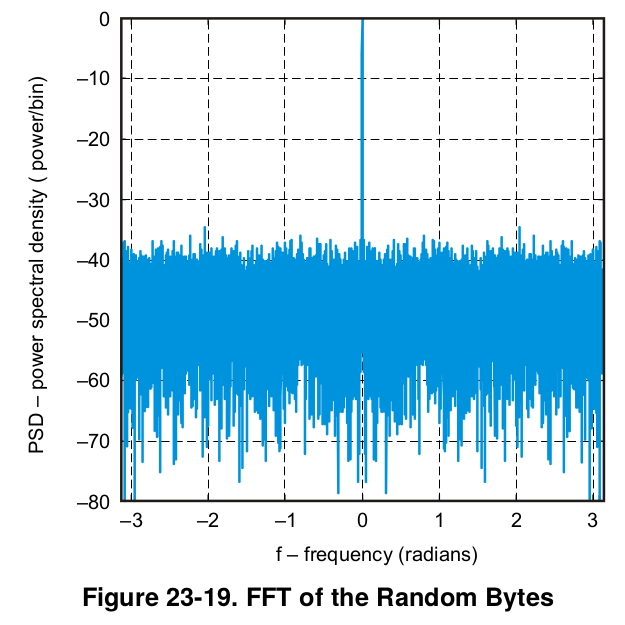
\includegraphics[width=2.5in]{fig/CC2538_Seed1.png}
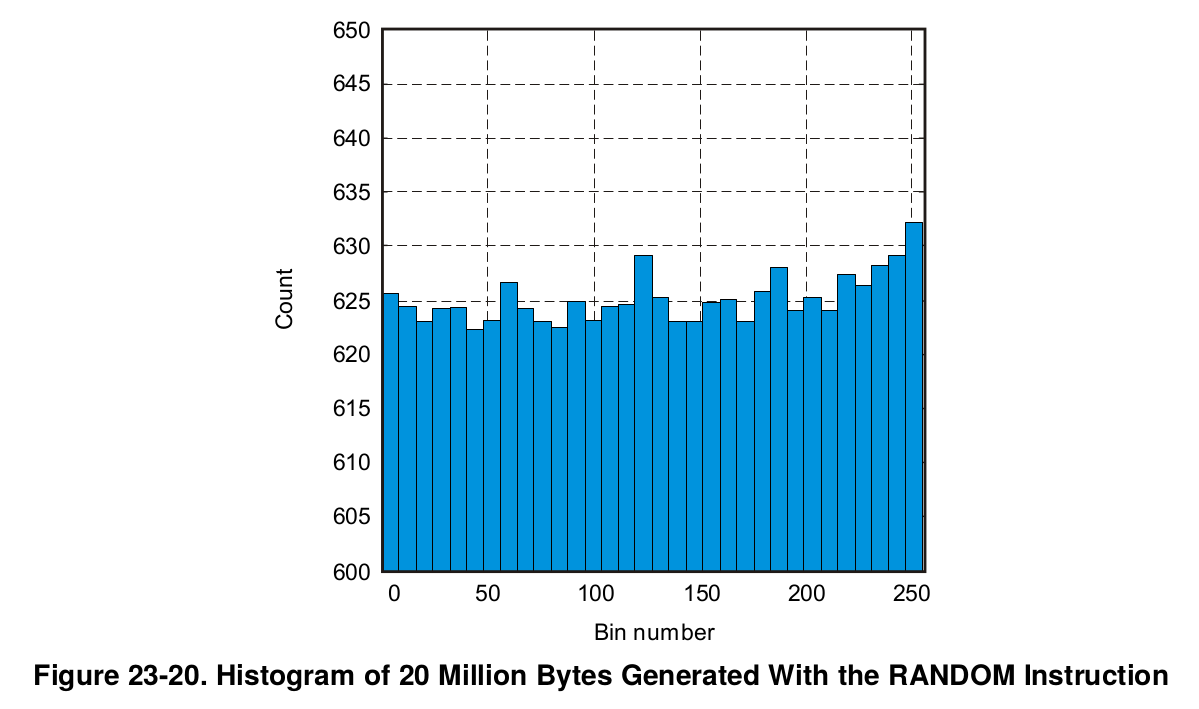
\includegraphics[width=2.5in]{fig/CC2538_Seed2.png}
\caption{RF core seeding result, from CC2538 User's Guide}
\label{SeedResult}
\end{figure}

To further verify the randomness of this seeding method, we applied the NIST Statistical Test Suite\cite{NISTTest} on 13263600 bits sampled by this seeding method using our application in \cite{prngtest}. Since each read to RFRND generates only $1$ bit, we concatenated all bits into one bit stream of length $13263600$. The bits has passed all tests in the NIST test suite, with $P(0) = 0.49995001$ and $P(1) = 0.50004999$. The full report and raw data are applicable at \cite{prngtest}.

Despite the good randomness of the seed, sampling from RF noise remains sceptical from a security perspective as such physical source can be easily tampered remotely by sending signal wave to the device.

The released documents did not explain further details of how the output of IF\_ADC in the receive I/Q channels translated to random bits. We have neither found any open document describes  the RF design of CC2538. 

However, we noticed the same RNG design has been applied on several product in TI's SimpleLink\texttrademark series. Some of them provided better explanation of their design of RF core and RNG which could be a hint to CC2538. In CC2430 user manual\cite{CC2430Manual}, we found a description of the RF core, shown in \Cref{CC2430RF}.

\begin{figure}[!t]
\centering
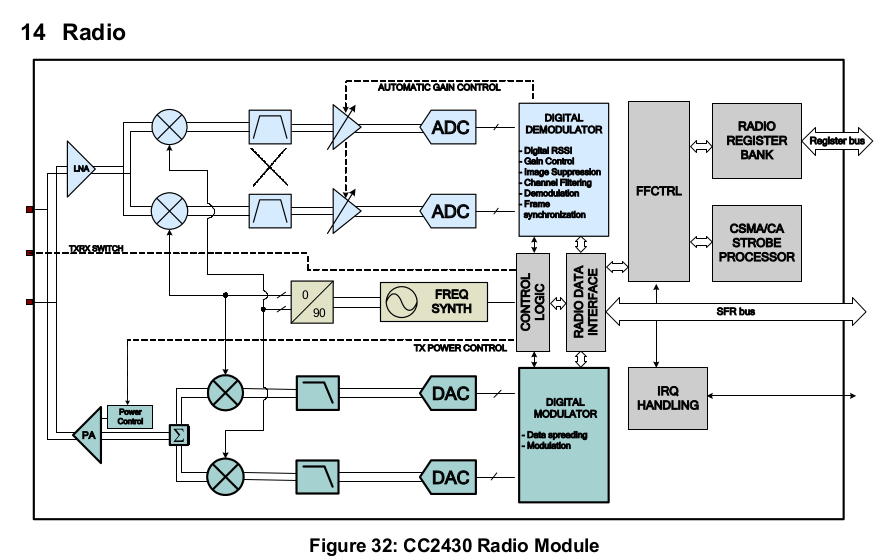
\includegraphics[width=2.5in]{fig/CC2430_Radio.png}
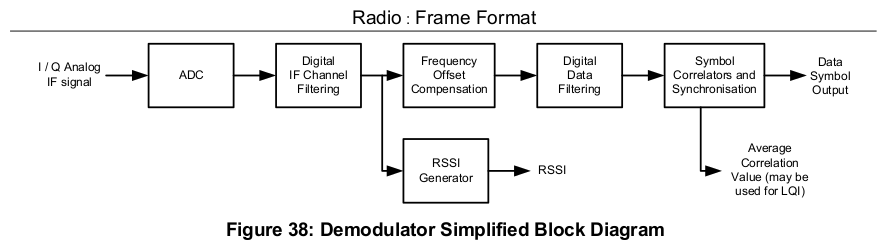
\includegraphics[width=2.5in]{fig/CC2430_Demodulator.png}
\caption{CC2430 RF Design, from CC2430 user manual\cite{CC2430Manual}}
\label{CC2430RF}
\end{figure}

\Cref{CC2430RF} suggests that the input analogue signal to IF\_ADC has went through the following components:
\begin{itemize}
	\item Low Noise Amplifier (LNA) which amplifies the signal.
	\item Mixer which down converts the signal frequency. The Frequency Synthesiser is used as the local oscillator.
	\item Band pass filter which filters out the out of band signals.
	\item The Automatic Gain Control (AGC) circuit which further adjusts the signal strength to the input level of ADC.
\end{itemize}

CC2520 Data Sheet\cite{CC2520Manual} explains the random bit is actually the Least Significant Bit (LSB) from ADC: (Section 24 in \cite{CC2520Manual})
\begin{quote}
Single random bits from either the I or Q channel (configurable) can be output on GPIO pins at a rate of 8MHz. One can also select to xor the I and Q bits before they are output on a GPIO pin. These bits are taken from the least significant bit in the I and/or Q channel after the decimation filter in the demodulator.
\end{quote}

A block diagram is also provided, as shown in \Cref{CC2520RFRND}.
\begin{figure}[!t]
\centering
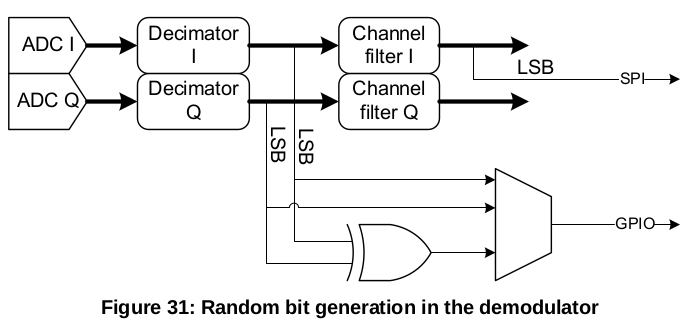
\includegraphics[width=2.5in]{fig/CC2520_RNG.png}
\caption{CC2520 RNG Design, from CC2520 user manual\cite{CC2520Manual}}
\label{CC2520RFRND}
\end{figure}

Interestingly, we noticed that CC2538, CC2520, CC253X and CC2540/41 reported exactly the identical randomness test result in their user manuals (\cite{CC2538Manual} \cite{ CC2520Manual} \cite{CC2530Manual}). This suggests they are very likely to have the same seeding design.

Assuming the same design has been applied to CC2538, it would explained the nice randomness of the seeding method. Denote $V$ as analogue RF signal and $N$ as noise, the analogue input to the ADC $V_{in}$ can be represented as:
\begin{equation}
V_{in} = V + N
\end{equation}

The noise $N$ can be induced by multiple sources in practice, including:
\begin{itemize}
\item Noise produced by the signal source.
\item Environmental noise.
\item Noise induced by the components in the device itself.
\end{itemize}
In practice, manipulating the noise could be difficult.

The random bit $b$ can be represented as:
\begin{equation} \label{RNDOutput}
b = LSB(V_{in}) = LSB(V + N)
\end{equation}
where $LSB() \in \{0,1\}$ represents the operation of taking the LSB of A/D conversion output.

Observing \Cref{RNDOutput}, one thing to be noticed is that any difference in $V_{in}$ larger than the scale of ADC, i.e. the voltage represented by its LSB, could flip $b$. According to CC2538 data sheet\cite{CC2538Datasheet}, the receiver can be sensitive to signals down to $-97dBm$ (typical value with $T_A = 25^{\circ}C$, $V_{DD} = 3V$ and $f_{C} = 2440MHz$). On the other hand, the typical environmental noise in our experimental environment, which is a typical office with multiple noise sources such as  WiFi, smart phones, etc, is about $-92dBm$ which is significantly higher than the receiver sensitivity. We consider the result of the randomness test as an evidence to this sampling method.

\section{Biasing Seed by Radio Jamming}
At a first glance one way to bias the seed is to generate a predictable $V_{in}$. \Cref{RNDOutput} indicates that the random bit $b$ is jointly determined by the signal $V$ and noise $N$. Even though $V$ can be viewed as being controlled by the adversary, manipulating $N$ turns out to be difficult in practice. For instance, noises accumulated by different amplification stages are physically inevitable. Hence fixing $V_{in}$ does not seem to be easily achievable in practice.

Therefore an alternative attempt is to provide the RF with an illegal $V_{in}$. Two methods are considered in our experiments:
\begin{itemize}
	\item Saturation. This method attempts to provide the RF with a strong signal that is above its acceptance level.
	\item Decimation. This method attempts to provide the RF with a weak signal that is beneath its acceptance level.
\end{itemize}

Ideally we expect these illegal inputs will trigger the ADC into a fault state which could potentially result into a predictable output and thus predictable $b$. But in practice, decimation does not seem practical for the same reason that noises induced by the circuits themself is physically inevitable. This made saturation the only viable option.

Meanwhile, the undisclosed circuit design of the device also poses a great difficulty in our experiments as without knowledge of the exact circuit designed it would be difficult to the deduce the most effective signal as well as to predict the outcome. We have only performed black box experiments on OpenMote which is a CC2538 based SoC.

\subsection{Sine wave signal}

\subsection{Sawtooth sine wave signal}

\subsection{Pulse signal}

\section{Conclusion}
In this paper we presented a study on the RNG design of CC2538. First, we revised the problem that using a 16 bit LFSR as PRNG is a bad idea and demonstrated how this design flaw can be exploited to break DTLS running on these devices. Secondly we presented a study to its seeding method and showed how such it could be remotely tampered by an adversary sending jamming signal to the device.

In fact the same RNG design has also been adopted many other products in the CC series including CC2420\cite{CC2420Manual}, CC2430\cite{CC2430Manual}, CC2520\cite{CC2520Manual} and CC253X, CC2540/41 series\cite{CC2530Manual}. We imagine all these products suffer the same problems. Fortunately the latest CC26XX/CC13XX\cite{CC26XXManual} has abandoned this design and implemented a dedicated RNG which TI describes as: (Chapter 16 in CC26XX/CC13XX Manual\cite{CC26XXManual})
\begin{quote}
The true random number generator (TRNG) module provides a true, nondeterministic noise source for the
purpose of generating keys, initialization vectors (IVs), and other random number requirements. The
TRNG is built on 24 ring oscillators that create unpredictable output to feed a complex nonlinear
combinatorial circuit. That post-processing of the output data is required to obtain cryptographically secure
random data.
\end{quote}

We sincerely hope this TRNG will provide the future IoT applications a secure RNG.

\section{Acknowledgement}
We have many thanks to (alphabetically) George Oikonomou for providing us much help in Contiki OS and the OpenMote devices, Geoff Hilton who helped us on RF designs and Jake Longo Galea who offered many signal processing advises.
\section{Related Source Code}

Source code related to this paper can be found at \cite{cc2538rng}. The repository contains all source file to reproduce the experiments done in this paper, including:
\begin{itemize}
	\item \textbf{prngtest}: Contiki application that iterates the CC2538 PRNG.
	\item \textbf{genr.py} and \textbf{secp256r1mult}: Tools to generate the EC key pair lookup table for CC2538 PRNG.
	\item \textbf{cc2538seed}: Contiki application that samples the RF seed for CC2538.
	\item \textbf{biasseed.py}: Implementation of the strong constant signal for HackRF One.
\end{itemize}

Detail usage documented in readme.txt. %Only included for author's version.

\bibliographystyle{IEEEtran}
\bibliography{references}

\appendix
\chapter{OrderFlavour-Length leakage channel}
\label{OrderFlavour leakage channel}

In this application, the joint probability of $Order$ and $Flavour$ are simply the product of their marginal probability. However, since “ESPRESSO” will always followed by $Flavour$ of of both degree of SUGAR and MILK being $0$(see  \Cref{ESPRESSO}); hence
\begin{eqnarray*}
P(x_1, x_2 | \text{“ESPRESSO”}) = 
	\begin{cases}
	1 &\text{if } x_1 = x_2 = 0\\
	0 &\text{otherwise}
	\end{cases}
\end{eqnarray*}

Therefore
\begin{eqnarray*}
P(\text{“ESPRESSO”}, x_1, x_2 ) = 
	\begin{cases}
	1/4 &\text{if } x_1 = x_2 = 0\\
	0 &\text{otherwise}
	\end{cases}
\end{eqnarray*}

\end{document}
